\documentclass[a4paper,12pt]{article} % добавить leqno в [] для нумерации слева
\usepackage[a4paper,top=1.3cm,bottom=2cm,left=1.5cm,right=1.5cm,marginparwidth=0.75cm]{geometry}
%%% Работа с русским языком
\usepackage{cmap}					% поиск в PDF
\usepackage{mathtext} 				% русские буквы в фомулах
\usepackage[T2A]{fontenc}			% кодировка
\usepackage[utf8]{inputenc}			% кодировка исходного текста
\usepackage[english,russian]{babel}	% локализация и переносы
\usepackage{multirow}

\usepackage{graphicx}

\usepackage{wrapfig}
\usepackage{tabularx}

\usepackage{hyperref}
\usepackage[rgb]{xcolor}
\hypersetup{
colorlinks=true,urlcolor=blue
}

%%% Дополнительная работа с математикой
\usepackage{amsmath,amsfonts,amssymb,amsthm,mathtools} % AMS
\usepackage{icomma} % "Умная" запятая: $0,2$ --- число, $0, 2$ --- перечисление

%% Номера формул
\mathtoolsset{showonlyrefs=true} % Показывать номера только у тех формул, на которые есть \eqref{} в тексте.

%% Шрифты
\usepackage{euscript}	 % Шрифт Евклид
\usepackage{mathrsfs} % Красивый матшрифт

%% Свои команды
\DeclareMathOperator{\sgn}{\mathop{sgn}}

%% Перенос знаков в формулах (по Львовскому)
\newcommand*{\hm}[1]{#1\nobreak\discretionary{}
{\hbox{$\mathsurround=0pt #1$}}{}}

%% Графики
\usepackage{tikz}
\usepackage{pgfplots}
\pgfplotsset{compat=1.9}

\date{\today}

\begin{document}

\begin{titlepage}
	\begin{center}
		{\large МОСКОВСКИЙ ФИЗИКО-ТЕХНИЧЕСКИЙ ИНСТИТУТ (НАЦИОНАЛЬНЫЙ ИССЛЕДОВАТЕЛЬСКИЙ УНИВЕРСИТЕТ)}
	\end{center}
	\begin{center}
		{\large Физтех-школа прикладной математики и информатики}
	\end{center}
	
	
	\vspace{4.5cm}
	{\huge
		\begin{center}
			{\bf Отчёт о выполнении лабораторной работы 3.3.1}\\
			Измерение удельного заряда электрона
		\end{center}
	}
	\vspace{1cm}
	\begin{center}
		{\large Соболевский Федор Александрович \\
			\vspace{0.2cm}
			Б05-111}
	\end{center}
	\vspace{8cm}
	\begin{center}
		Сентябрь 2022
	\end{center}
\end{titlepage}

\section{Аннотация}

В данной работе исследовано воздействие магнитного поля на заряженные частицы - в частности, на электроны. По величине и характеру данного воздействия определён удельный заряд электрона. Данная величина измерена двумя различными способами: методом магнитной фокусировки и методом магнетрона. По отклонению результатов экспериментов от табличных значений и по величине погрешности оценена применимость данных методов для вышеописанных измерений.

\section{Теоретические сведения}

\subsection{Метод магнитной фокусировки}

На заряд, движущийся со скоростью $v$ в магнитном поле $B$, действует сила Лоренца:

\begin{equation}
    \mathbf{F} = q\mathbf{v}\times\mathbf{B}.
\end{equation}

Движущаяся под углом к полю заряженная частица описывает винтовую линию вокруг направления вектора магнитной индукции, радиус которой равен

\begin{equation}
    r_B = \frac{mv_\bot}{qB}, 
\end{equation}

где $v_\bot$ - перпендикулярная составляющая скорости, $m$ - масса заряженной частицы, $q$ - её заряд. При этом параллельная составляющая скорости $v_\parallel$ остаётся постоянной, т.к. она перпендикулярна действующей на неё силе. За время прохождения электроном одного витка спирали (т.е. за \textit{циклотронный период}) заряд сместится вдоль магнитного поля на расстояние $L$:

\begin{equation}
    L = v_\parallel T_B = \frac{2\pi v \text{cos }\alpha}{\frac{e}{m}B},
\end{equation}

где $\alpha$ - угол между вектором скорости и направлением поля. При достаточно малых $\alpha$ cos $\alpha \approx 1$ и

\begin{equation}
    L \approx \frac{2\pi v}{\frac{e}{m}B}.
    \label{spiralStep}
\end{equation}

При малых углах расстояние $L$ не зависит от $\alpha$, и все электроны после одного оборота сфокусируются в одной точке. Таким образом, зная величину $L$ и магнитной индукции $B$, можно вычислить $e/m$ - удельный заряд электрона.

\subsubsection{Экспериментальная установка}

\begin{figure}
    \centering
    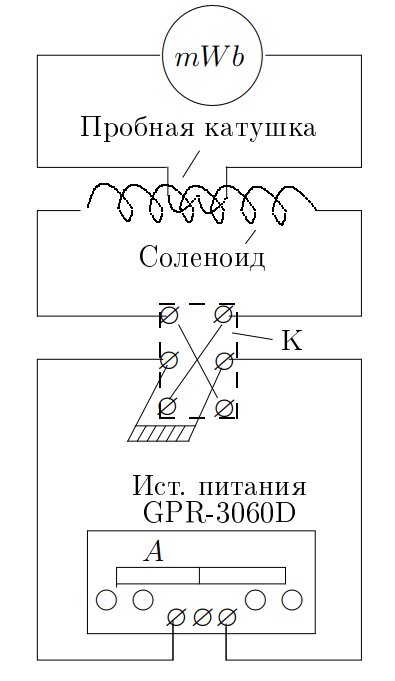
\includegraphics[width = 0.35\textwidth]{setupA.png}
    \caption{Схема установки для измерений по методу магнитной фокусировки}
    \label{fig:setupA}
\end{figure}

На рис. \ref{fig:setupA} изображена схема установки для измерения удельного заряда электрона методом магнитной фокусировки. Основной её частью является электронный осциллограф, трубка которого вытянута и установлена в длинном соленоиде, создающем магнитное поле, направленной вдоль оси трубки. Пучок эмитированных с катода электронов ускорялся анодным напряжением порядка ~1 кВ и пропускался через две диафрагмы для получения пучка частиц с малой расходимостью $(\Delta \alpha \ll 1)$ и малым разбросом скоростей относительно значения 

\begin{equation}
    v_\parallel = \sqrt{\frac{2eU_A}{m}}.
    \label{eSpeed}
\end{equation}

Данное значение получено из закона сохранения энергии.

В магнитном поле соленоида электроны двигаются по спиралям с практически равным шагом L, встречаясь на расстояниях $nL$, $n = $1, 2, 3... В этих точках изображение пучка на экране будет стягивается в точку. Зная величину магнитного поля соленоида $B_\Phi$, из \eqref{spiralStep} и \eqref{eSpeed} получим выражение для удельного заряда электрона:

\begin{equation}
    \frac{e}{m} = \frac{8\pi^2 U_A}{L^2} \cdot \frac{n^2}{B_\Phi^2(n)}.
    \label{finalA}
\end{equation}

Анодное напряжение $U_A$ измерялось с помощью вольтметра, величина магнитного поля изменялась амперметром источника тока и измерялась милливеберметром.

\subsection{Метод магнетрона}

Метод магнетрона заключается в исследовании движения электрона в скрещенных электрическом и магнитном полях. Такая конфигурация реализуется в магнетронах - генераторах электромагнитных колебаний сверхвысоких частот.

\begin{figure}
    \centering
    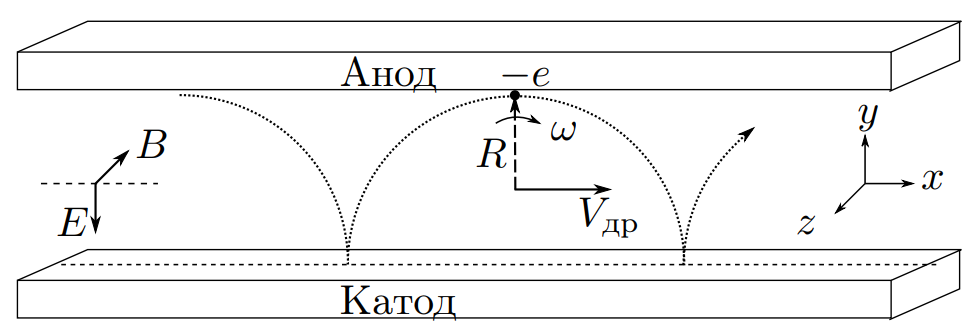
\includegraphics[width = 0.6\textwidth]{electronMovement.png}
    \caption{Движение заряда в скрещенных полях}
    \label{fig:electronMovement}
\end{figure}

На рис. \ref{fig:electronMovement} схематично изображена траектория движения электрона в скрещенных полях в плоском магнетроне - катоде и аноде, пространство между которыми заполнено вакуумом. От величины магнитного поля зависит искривление траектории движения электронов между заряженными пластинами. До некоторого критического значения $B_\text{кр}$ практически все вылетающие с катода электроны будут попадать на анод, после - будут возвращаться обратно на катод.

Рассчитаем критическое магнитное поле для плоского конденсатора с электрическим полем $E$ и магнитным полем $B$. Движение электрона в нём описывается системой уравнений:

\begin{equation*}
    \begin{cases}
    \dot{v_x} = \omega_B v_y, \\
    \dot{v_y} = \frac{e}{m}E - \omega_B v_x, \\
    \dot{v_z} = 0.
    \end{cases}
\end{equation*}

Если начальная скорость равна нулю (начальные условия $x(0) = y(0) = 0$, $v_x(0) = v_y(0) = 0$), то из уравнений следует, что траектория движения будет циклоидой:

\begin{equation}
    x = Vt - R\text{sin }\omega_B t \text{,     } y = R(1 - \text{cos}\omega_B t),
\end{equation}

где $V = E/B$ - дрейфовая скорость, $R = V/\omega_B = Em/(eB^2)$. Касание анода происходит при $2R = h$, где $h$ - расстояние между катодом и анодом. Этому значению соответствует критическое поле

\begin{equation}
    B_\text{кр} = \frac{\sqrt{2U}}{h\sqrt{e/m}},
\end{equation}

где $U = Eh$ - напряжение между пластинами. Отсюда удельный заряд

\begin{equation}
    \frac{e}{m} = \frac{2U}{B_\text{кр}^2 h^2}.
\end{equation}

\begin{figure}
    \centering
    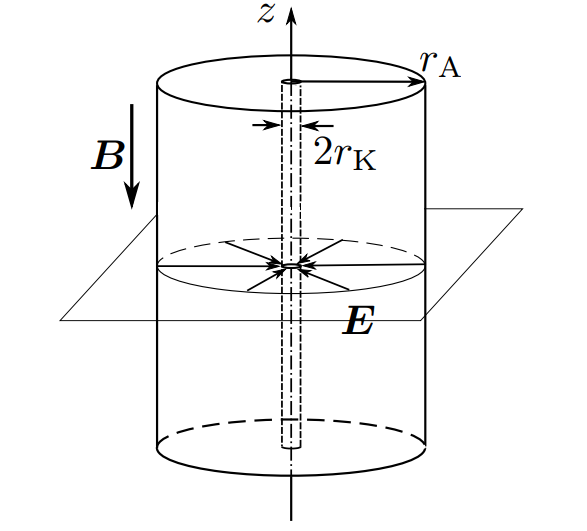
\includegraphics[width = 0.45\textwidth]{sphericMagnetron.png}
    \caption{Схема устройства двухэлектродной лампы}
    \label{fig:sphericMagnetron}
\end{figure}

В случае сферического магнетрона - двухэлектродной лампы, помещенной в магнитном поле соленоида (см. рис. \ref{fig:sphericMagnetron}), траектории частиц будут несколько отличаться от рассмотренного случая, однако их качественные особенности сохранятся, а выражение будет отличаться лишь численным коэффициентом. Проведя вычисления, аналогичные вышеприведённым, для случая цилиндрической лампы, получим окончательное выражение для удельного заряда:

\begin{equation}
    \frac{e}{m} = \frac{8U_A}{B_\text{кр}^2 r_A^2},
    \label{finalB}
\end{equation}

где $r_A$ - радиус анода.

\subsubsection{Экспериментальная установка}

\begin{figure}
    \centering
    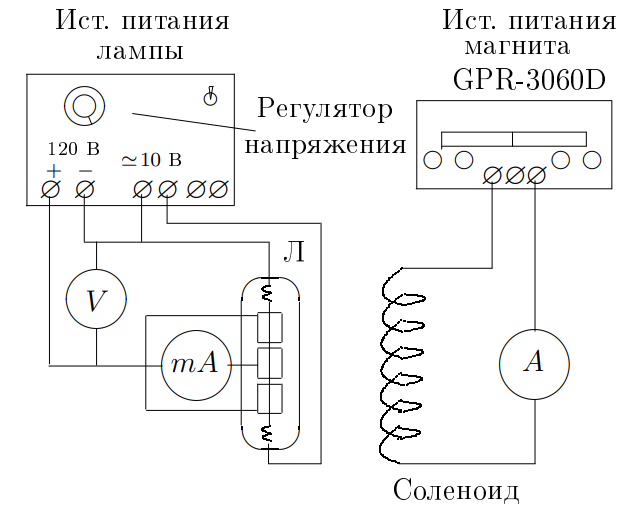
\includegraphics[width = 0.6\textwidth]{setupB.png}
    \caption{Схема установки для измерения удельного заряда методом магнетрона}
    \label{fig:setupB}
\end{figure}

Схема установки изображена на рис. \ref{fig:setupB}. Анод лампы состоит из трёх немагнитных металлических цилиндров одинакового диаметра. Крайние электрически изолированы и служат для устранения краевых эффектов на торцах среднего цилиндра, ток с которого используется при измерениях. В качестве анода используется тонкая вольфрамовая проволока, расположенная по оси цилиндров. Катод разогревается проходящим через него переменным током, создаваемым стабилизированным источником питания. На анод подаётся постоянное напряжение от регулируемого источника, измеряемое вольтметром. Ток через среднюю секцию анода измеряется миллиамперметром. Лампа закреплена в соленоиде, ток в который подаётся с независимого источника и измеряется амперметром. Индукция магнитного поля в соленоиде рассчитывается по току в обмотке с помощью указанного на установке коэффициента.

В реальных условиях невозможно обеспечить полную коаксиальность анода и катода, вектор индукции магнитного поля всегда несколько наклонён по отношению к катоду и т.д. Это приводит к сглаживанию кривой $I_A(B)$ (см. рис. \ref{fig:IA}). Однако в хорошо собранной установке перелом графика достаточно резкий, чтобы по нему определить критическое значение индукции.

\begin{figure}
    \centering
    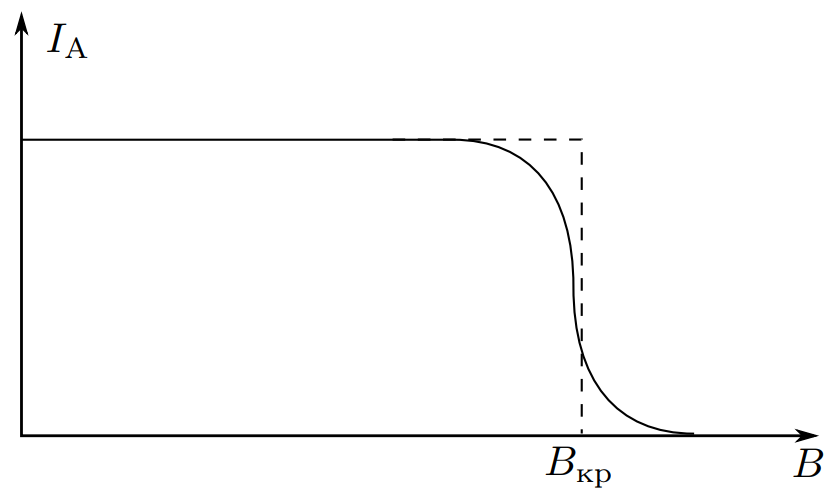
\includegraphics[width = 0.49\textwidth]{IA.png}
    \caption{Зависимость анодного тока от индукции магнитного поля в соленоиде}
    \label{fig:IA}
\end{figure}

\section{Оборудование и инструментальные погрешности}

\textbf{В работе использовались:} А) электронно-лучевая трубка с блоком питания, соленоид, регулируемый источник постоянного тока, вольтметр, милливеберметр, ключ; Б) электронная лампа с цилиндрическим анодом, регулируемый источник постоянного тока, соленоид, вольтметр, два амперметра.

\textbf{Инструментальные погрешности:}

А) Метод магнитной фокусировки:
\begin{itemize}
    \item Амперметр источника тока: $\Delta_I = 0,01$ А;
    \item Вольтметр источника тока: $\Delta_U = 0,1$ В;
    \item Вольтметр ускоряющего напряжения: $\Delta_{U_A} = 0,01$ кВ;
    \item Милливеберметр: $\Delta_B = 0,05$ мВб.
\end{itemize}

Б) Метод магнетрона:
\begin{itemize}
    \item Миллиамперметр: $\Delta_{I_a} = 0,01$ мА;
    \item Амперметр соленоида: $\Delta_{I_m} = 0,002$ мА;
    \item Вольтметр: $\Delta_U = 0,5$ В.
\end{itemize}

\section{Результаты измерений и обработка экспериментальных данных}

\subsection{Измерения методом магнитной фокусировки}

\subsubsection{Калибровка милливеберметра}

Перед началом измерений путём измерения магнитного потока $\Phi$ была установлена зависимость индукции магнитного поля соленоида от тока в ней. Величину индукции магнитного поля можно найти как $B = \Phi/(SN)$, где $SN = 3000$ см$^2$ для использованной катушки. Полученные значения представлены в таблице \ref{tab:calibration}. Калибровочная прямая изображена на рис. \ref{graph:calibration}. По углу наклона калибровочной прямой установлено, что ток в 1 А соответствует величине магнитной индукции 4,6 $\pm$ 0.2 мТл.

\begin{table}
\centering
\begin{tabular}{|c|c|c|c|c|c|}
\hline
$I$, А & $\Phi$, мВб & $B_\Phi$, мТл & $I$, А & $\Phi$, мВб & $B_\Phi$, мТл \\ \hline
0,5 & 0,7 & 2,3 & 0,5 & 0,6 & 2,0 \\ \hline
1,0 & 1,3 & 4,3 & 1,0 & 1,3 & 4,3 \\ \hline
1,5 & 2,0 & 6,7 & 1,5 & 2,0 & 6,7 \\ \hline
2,0 & 2,7 & 9,0 & 2,0 & 2,6 & 8,7 \\ \hline
2,5 & 3,4 & 11,3 & 2,5 & 3,4 & 11,3 \\ \hline
3,0 & 4,1 & 13,7 & 3,0 & 4,1 & 13,7 \\ \hline
\end{tabular}
\caption{Калибровочные значения для милливеберметра}
\label{tab:calibration}
\end{table}

\begin{figure}
\centering
\resizebox {0.55\textwidth} {!} {
\begin{tikzpicture}
\begin{axis}[ xlabel = {$I$, А}, ylabel = {$B$, мТл}, xmin = 0, xmax = 3.5, ymin = 0, ymax = 14.5]
\addplot[color=black, mark=x, only marks] coordinates{
(0.5, 2.3)
(0.5, 2)
(1, 4.3)
(1.5, 6.7)
(2, 9)
(2, 8.7)
(2.5, 11.3)
(3, 13.7)
};
\addplot[color=blue] {4.55*x};
\end{axis}
\end{tikzpicture}
}
\caption{Калибровочная прямая для милливеберметра}
\label{graph:calibration}
\end{figure}

\subsubsection{Определение фокусирующего тока и вычисление удельного заряда}

Далее в ходе работы было измерено по 5 фокусирующих значений тока и соответствующих им величин индукции магнитного поля для каждого направления тока. Результаты представлены в таблице \ref{tab:focuses}. На рис. \ref{graph:focuses} изображён график зависимости фокусирующей индукции поля от номера фокуса. Отсюда можем найти значение $B_\Phi / n = 2,53 \pm 0,03$ мТл.

\begin{table}
\centering
\begin{tabular}{|c|c|c|c|c|c|}
\hline
$n$ & $I$, А & $B_\Phi$, мТл & $n$ & $I$, А & $B_\Phi$, мТл \\ \hline
1 & 0,55 & 2,5 & 1 & 0,54 & 2,5 \\ \hline
2 & 1,10 & 5,1 & 2 & 1,10 & 5,1 \\ \hline
3 & 1,65 & 7,8 & 3 & 1,69 & 7,8 \\ \hline
4 & 2,21 & 10,4 & 4 & 2,25 & 10,4 \\ \hline
5 & 2,69 & 12,4 & 5 & 2,77 & 12,7 \\ \hline
\end{tabular}
\caption{Значения фокусирующего тока и соответствующие им значения индукции магнитного поля}
\label{tab:focuses}
\end{table}

\begin{figure}
\centering
\resizebox {0.55\textwidth} {!} {
\begin{tikzpicture}
\begin{axis}[ xlabel = {$n$ фокуса}, ylabel = {$B$, мТл}, xmin = 0, xmax = 5.5, ymin = 0, ymax = 13.5]
\addplot[color=black, mark=x, only marks] coordinates{
(1, 2.5)
(2, 5.1)
(3, 7.6)
(3, 7.8)
(4, 10.2)
(4, 10.4)
(5, 12.7)
(5, 12.4)
};
\addplot[color=blue] {2.53*x};
\end{axis}
\end{tikzpicture}
}
\caption{Зависимость индукции магнитного поля катушки от номера фокуса}
\label{graph:focuses}
\end{figure}

Зная ускоряющее напряжение $U_a = 800 \pm 10$ В и длину трубки осциллографа $l = 0,265$ м, можно вычислить по формуле \eqref{finalA} значение удельного заряда электрона:

\begin{equation}
    \frac{e}{m} = \frac{8\pi^2 U_a}{l^2}\cdot(\frac{n}{B_\Phi})^2 \approx (1,41 \pm 0,08) \cdot 10^{11} \text{ Кл/кг}.
\end{equation}

\subsection{Измерения методом магнетрона}

Для шести значений ускоряющего напряжения $U_a$ в диапазоне 70-120 В измерена зависимость анодного тока от тока в катушке и соответствующей ему магнитной индукции. Для использованной в опыте катушки справедливо $B_m = kI_m$, где $k = 2,8 \cdot 10^{-2}$ Тл/А. На рис.  изображены полученные графики зависимости анодного тока от индукции магнитного поля в соленоиде. По ним определены соответствующие значения критической индукции поля. Для каждого значения по формуле \eqref{finalB} найдено значение удельного заряда. Усреднив, получаем окончательный ответ:

\begin{itemize}
    \item $e/m = (1,33 \pm 0.16)\cdot 10^{11}$ Кл/кг. 
\end{itemize}

\begin{figure}
\centering
\resizebox {0.86\textwidth} {!} {
\begin{tikzpicture}
\begin{axis}[ xlabel = {$B$, мкТл}, ylabel = {$I_a$, мкА}, xmin = 0, xmax = 8, ymin = 0, ymax = 500, minor x tick num=10]
\addplot[color=black, mark=x] coordinates{
(0, 480)(1.68, 444)(2.24, 400)(2.8, 344)(3.36, 284)(3.92, 112)(4.48, 24)(5.04, 12)(5.6, 4) 
};
\addplot[color=blue, mark=*] coordinates{
(0, 468)(1.68, 452)(2.24, 400)(2.8, 380)(3.36, 284)(3.92, 192)(4.48, 32)(5.04, 20)(5.6, 8) 
};
\addplot[color=purple, mark=o] coordinates{
(0, 448)(2.24, 416)(2.8, 384)(3.36, 332)(3.92, 244)(4.48, 84)(5.04, 24)(5.6, 16)(6.16, 8) 
};
\addplot[color=red, mark=square] coordinates{
(0, 448)(2.24, 448)(2.8, 392)(3.36, 368)(3.92, 308)(4.48, 204)(5.04, 60)(5.6, 24)(6.16, 12)(6.72, 8) 
};
\addplot[color=green, mark=triangle] coordinates{
(0, 436)(2.8, 404)(3.36, 396)(3.92, 344)(4.48, 284)(5.04, 180)(5.6, 44)(6.16, 24)(6.72, 12)(7.28, 4) 
};
\addplot[color=gray, mark=star] coordinates{
(0, 440)(2.8, 416)(3.36, 400)(4.48, 344)(5.04, 272)(5.6, 88)(6.16, 28)(6.72, 16)(7.28, 8)(7.84, 4) 
};
\legend{70 В, 80 В, 90 В, 100 В, 110 В, 120 В}
\end{axis}
\end{tikzpicture}
}
\caption{Зависимость анодного тока от индукции магнитного поля при разных ускоряющих напряжениях}
\label{graph:anodeCurrents}
\end{figure}

\section{Обсуждение результатов и выводы}

В данной работе получены следующие значения удельного электрического заряда электрона:

\begin{itemize}
    \item \textbf{Методом магнитной фокусировки:} $e/m = (1,41 \pm 0,08)\cdot 10^{11}$ Кл/кг;
    \item \textbf{Методом магнетрона:} $e/m = (1,33 \pm 0,16)\cdot 10^{11}$ Кл/кг.
\end{itemize}

Табличное значение удельного заряда $(e/m)_\text{теор} = 1,76\cdot 10^{11}$ Кл/кг. Полученные в опытах значения отклоняются от этого значения на 20-25\%. Такое отклонение говорит о том, что в нашей установке измеренная величина воздействия поля на движущийся заряд меньше теоретической. Это может быть объяснено дефектами данных установок, связанными с длительностью их эксплуатации, и неидеальностью лабораторных условий в сравнении с теоретической моделью.

Сравнение погрешностей полученных результатов говорит о том, что с предложенными в лаборатории приборами заметно лучшую точность измерений даёт метод магнитной фокусировки. Большая погрешность измерений вторым методом связана, прежде всего, с небольшой точностью миллиамперметра, с помощью которого был измерен ток через создающий магнитное поле соленоид. Для получения более точных результатов можно применить миллиамперметр с меньшей ценой деления.

Несмотря на погрешности и отклонение результатов от табличных значений, в ходе данной работы была получена правильная по порядку величина удельного заряда электрона, что говорит о справедливости применённых теоретических соотношений. 

\end{document}